\documentclass{statsmsc}

% Vim note: zo, zc and zm to open and close folds, and close all folds

% Commands {{{

\title{Title of the Thesis}
\author{FIRSTNAME LASTNAME}
\CID{01234567}
\supervisor{SUPERVISORNAME and COSUPERVISORNAME}
\date{1 May 2022}
%For today's date, use:
%\date{\today}
\logoimg{}


% THIS IS WHERE NEW COMMANDS CAN BE DEFINED
% commands below only used in the proof; otherwise can be deleted
\newcommand{\consta}{a}
\newcommand{\X}{X}
\newcommand{\EE}[1]{ \mathrm{E} [ #1 ] }
\newcommand{\inparenth}[1]{\left( #1 \right)}

% }}}

\begin{document}

%%%%% Heading %%%%%
% Heading {{{

% Generates the Title Page
\maketitle


% Generates plagiarism declaration
\declarationname{STUDENT'S NAME}
\declarationdate{DATE}
\declaration 


\begin{abstract}
    ABSTRACT GOES HERE
\end{abstract}

\begin{acknowledgements}
    ANY ACKNOWLEDGEMENTS GO HERE
\end{acknowledgements}

{\thispagestyle{plain}
    % TODO: Load hyperref so that ToC items are clickable
    \tableofcontents
}

% Glossary ?
{\chapter*{Notation}\thispagestyle{plain}
    $\boldsymbol{X}$ is a matrix

    $y$ is a vector
}

% Abbreviations
{\chapter*{Abbreviations}\thispagestyle{plain}
    \begin{acronym}[TDMA]
        \acro{DAIN}{Deep Adaptive Input Normalization}
        \acro{RDAIN}{Robust Deep Adaptive Input Normalization}
        \acro{EDAIN}{Extended Deep Adaptive Input Normalization}
        \acro{EDAIN-KL}{Extended Deep Adaptive Input Normalization, optimised with Kullback–Leibler divergence}
        \acro{BIN}{Bilinear Input Normalization}
        \acro{pdf}{probability density function}
        \acro{KL-divergence}{Kullbeck-Leibler divergence}
    \end{acronym}
}



% VERY IMPORTANT
% This command switches from Roman to Arabic numbering for main part of thesis
\mainmatter

% }}}

%%%%%%%%%%%%%%%%%%%%%%%%%%%%%%%%%%%%%%%%%%%%%%%%%%%%%%
\chapter{Introduction} %%%%     Introduction      %%%%
%%%%%%%%%%%%%%%%%%%%%%%%%%%%%%%%%%%%%%%%%%%%%%%%%%%%%%
% Introduction {{{

The introduction section goes here\footnote{Tip: write this section last.}.

% }}}

%%%%%%%%%%%%%%%%%%%%%%%%%%%%%%%%%%%%%%%%%%%%%%%%%%%%%%
\chapter{Background} %%%%        Background       %%%%
%%%%%%%%%%%%%%%%%%%%%%%%%%%%%%%%%%%%%%%%%%%%%%%%%%%%%%

TODO: introduction to this chapter

\section{Deep learning}% Deep learning
% Methods: Deep learning {{{
\label{sec:Deep learning}

TODO: write details

\subsection{Sequence models}%
\label{sub:Sequence models}


% }}}

\section{Data preprocessing}% Data preprocessing
% Methods: Data preprocessing {{{
\label{sec:Data preprocessing}

Origin pa

\cite{stanislav} does some data preprocessing for neural networks, and
\cite{nawi} also investigate the effect of data preprocessing on neural network.
Also looked at effect on classification performance by \cite{singh}.
Moreover, been studied as early as 1997 by \citep{preprocess_origin}.

% Static distribution transformations
\subsection{Static distribution transformations}% {{{
\label{sub:Static distribution transformations}


% }}}

% Adaptive distribution transformation
\subsection{Adaptive distribution transformations}% {{{
\label{sub:Adaptive distribution transformations}

\subsubsection{DAIN}%
\label{ssub:DAIN}

The \ac{DAIN} method, proposed by \cite{dain}.

\subsubsection{RDAIN}%
\label{ssub:RDAIN}

We have \cite{rdain}

\subsubsection{BiN}%
\label{ssub:BiN}

We have \cite{bin}

% }}}


% }}}


\section{Normalizing flows}% Normalizing flows
% Methods: Normalizing flows {{{
\label{sec:Normalizing flows}

TODO: write details

% }}}


%%%%%%%%%%%%%%%%%%%%%%%%%%%%%%%%%%%%%%%%%%%%%%%%%
\chapter{Methods} %%%%       METHODS         %%%%
%%%%%%%%%%%%%%%%%%%%%%%%%%%%%%%%%%%%%%%%%%%%%%%%%

TODO: introduction to this chapter

\section{EDAIN}% EDAIN
% Methods: EDAIN {{{
\label{sec:EDAIN-method}

% Topics of this section:
% * Illustrative diagram of the 4 layers, and the weights, justifying order of operations
% * Differences to DAIN, explaining batch awareness, and specifics of (amex) dataset worked with
% * Explaining the 3 parts:
%   * outlier removal: Inspired by winsorization, plot of curve for different values,to show how work
%   * scale&shift: able to generalise standard scaling
%   * power transform: should also work for negative and positive values, while being numerically stable

My first contribution is the \ac{EDAIN} layer. This adaptive preprocessing layer is inspired
by the likes of DAIN\_REF and BIN\_REF, but unlike the aforementioned methods, the
\ac{EDAIN} layer also supports normalizing the data in a \textit{batch-agnostic} fashion, whereas
the \ac{DAIN}, \ac{RDAIN} and \ac{BIN} layers are all \textit{batch-aware}.
Additionally, the \ac{EDAIN} layer extends the other layers with two new operations: An outlier
removal operation that is designed to reduce the negative impact of high-tail observations,
as well as a power-transform operation that is designed to transform non-normal data to be more
normal.

\subsection{Notation}%
\label{sub:Notation}


Let $\{\bfX^{(i)} \in \R^{d \times T};i=1,\dots,N\}$ denote a set of $N$ multivariate time-series,
each composed of $T$ $d$-dimensional feature vectors. We also let $\bfx_t^{(i)}\in \R^d$,
where $t=1,\dots,T$, denote the $t$th feature vector at time-step $t$ in the time-series.

\subsection{Architecture}%
\label{sub:Architecture}

% TODO: make figure, then finish this section...

An overview of the layer's architecture is shown in figure TODO\_FIG.
First, outlier removal. Then scale. Then shift. Then power transform.
This order because TODO.

TODO: explain comparison to DAIN, RDAIN and BIN, and how not batch-aware, but rather aims to
learn characteristics of global distribution, as it's the global distribution that might be
very irregular...

% TODO: should somewhere clearly specify that x is 3-dimensional, and all the
%       element-wise operations happen over the dimension axis
%       this can nicely be done by always writing x_t^{(i)} in the equations, since then
%       it's a 1D vector of dimensions d

% Outlier removal
\subsubsection{Outlier removal}% {{{
\label{ssub:Outlier removal}

Handling outliers and extreme values in the dataset can increase predictive performance if done
correctly (citation needed). Two common ways of doing this are omission and winsorization
\citep{winsorization}. With the former, observations that are deemed to be extreme are simply
removed during training. With the latter, all the data is still used, but observations lying
outside a certain number of standard deviation from the mean, or below or above certain
percentiles, are \textit{clamped down} to be closer to the mean or median of the data.
For example, if winsorizing data using 3 standard deviation, all values less than
$\mu-3\sigma$ are set to be exactly $\mu-3\sigma$. Similarly, the values above
$\mu+3\sigma$ are \textit{clamped} to this value. Winsorization can also be done using percentiles,
where common boundaries are the first and fifth percentiles \cite{winsorization}.
However, the type of winsorization, as well as the number of standard deviation
or percentiles to use, might depend on the dataset. Additionally, it might not
be necessary to winsorize the data at all if the outliers turn out to not
negatively affect performance. All this introduces more hyperparameters to tune
during modelling. The outlier removal presented here aims to automatically both determine
whether winsorization is necessary for a particular feature, and determine the threshold at
which to apply winsorization.

For input vector $\bfx \in \R^d$, the adaptive outlier removal operation is defined as:
\begin{equation}\label{eq:adaptive-outlier-removal}
    \bm\alpha' \odot \underbrace{\left(\bm\beta' \odot 
        \tanh\left\{(\bfx-\hat{\bm\mu}) \oslash \bm\beta'  \right\}+\hat{\bm\mu}
\right)}_{\text{smooth adaptive centred winsorization}}
    +\underbrace{\left(1-\bm\alpha' \right) \odot \bfx}_{\text{residual connection}},
\end{equation}
where $\odot$ is the element-wise multiplication, $\oslash$ is element-wise division,
$\bm\alpha' \in [0,1]^d$ is a parameter controlling how much winsorization to apply to each feature,
and $\bm\beta' \in [\beta_{\text{min}},\infty)^d$ controls the winsorization threshold for
each feature, that is, the maximum absolute value of the output, thus controlling the range of the
output. The effect of the two parameters is illustrated in \cref{fig:adaptive_outlier}.
The $\hat{\bm\mu}$ parameter is an estimate of the mean of the data, and is used
to ensure the winsorization is centred. When setting the \ac{EDAIN} layer in \textit{batch-aware}
mode, it is simply the mean of the batch:
\begin{equation}
    \hat{\mu}_k=\frac{1}{|\mathcal{B}| T} \sum_{i \in \mathcal{B}} \sum_{t=1}^T x_{j,k}^{(i)},
\end{equation}
while if using the \textit{batch-agnostic} mode, it is iteratively updated using a cumulative
moving average estimate at each forward pass of the layer. This is to better approximate the
global mean of the data.
The unknown parameters of the model are $\bm\alpha \in \R^d$ and $\bm\beta \in \R^d$, and they
are transformed into the constrained parameters $\bm\alpha'$ and $\bm\beta'$, as used in
\cref{eq:adaptive-outlier-removal} through the following element-wise mappings:
\begin{equation}
    \bm\alpha'=\frac{e^{\bm\alpha}}{1+e^{\bm\alpha}} \;\;\;\;\;\;\;\;\;
    \bm\beta'=\beta_{\text{min}}+e^{\bm\beta}.
\end{equation}
For ease of notation, we let $\mathbf{W}_1=(\bm\alpha, \bm\beta)$ denote the $2d$ unknown
parameters that are optimised for the adaptive outlier removal layer.

\begin{figure}
\begin{center}
    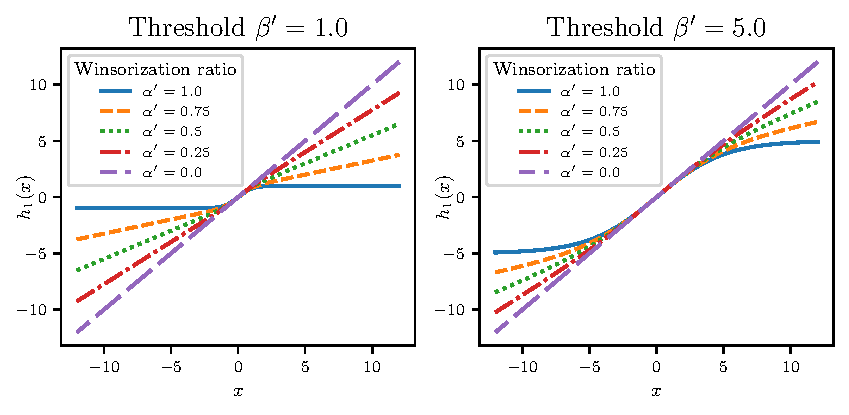
\includegraphics[scale=1.0]{figures/adaptive_outlier_removal.pdf}
\end{center}
\caption{Plot of the adaptive outlier removal operation for different combinations of parameter 
values for $\alpha'$ and $\beta'$.}
\label{fig:adaptive_outlier}
\end{figure}


% }}}

% Scale and shift
\subsubsection{Scale and shift}% {{{
\label{ssub:Scale and shift}

% TODO: reformulate this section to combine both of the layers in the below equation,
%       as that is more readable, then compare batch-aware and batch-agnostic versions,
%       and as example, write how the batch-agnostic one can generalise standard scaling...

The adaptive shift and scale layer, combined, simply performs the operation
\begin{equation}\label{eq:adaptive-scale-shift}
    (\bfx \oplus \bm\gamma) \odot \bm\lambda,
\end{equation}
with input $\bfx$ and unknown parameters $\bm\gamma \in \R^d$ and $\bm\lambda \in (0,\infty)^d$ when the \ac{EDAIN} is set
to batch-agnostic mode. This makes the scale-and-shift layer a generalised version of
Z-score scaling, or standard scaling, as setting
\begin{equation}
    \bm\gamma:=-\frac{1}{N T}  \sum^{N}_{i=1} \sum^{T}_{t=1} \bfx_{t}^{(i)}
\end{equation}
and
\begin{equation}
    \bm\lambda:=\left( \frac{1}{N T} \sum^{N}_{i=1} \sum^{T}_{t=1} \left(\bfx_{t}^{(i)}\oplus \bm\gamma\right)^2  \right)^{-1}
\end{equation}
makes the operation in \cref{eq:adaptive-scale-shift} equivalent to Z-score scaling.
This \textit{batch-agnostic} mode is useful if the distribution is similar across batches
and constitute a global unimodal distribution that should be centred.

However, some datasets might have multiple modes arising from significantly different
data generation mechanisms. Attempting to scale and shift each batch to a global mean and
standard deviation might hurt performance in such cases. Instead, CITE\_AUTHOR\_DAIN propose
basing the scale and shift on a \textit{summary representation} of the current batch, allowing
each batch to be normalized according the specific mode that batch of data might have come from.
This gives
\begin{equation}
    (\bfx \oplus [\bm\gamma \odot \mu_{\bfx}]) \odot [\bm\lambda \odot \sigma_{\bfx}],
\end{equation}
where the summary representations $\sigma_{\bfx}$ and $\mu_{\bfx}$ are computed through reduction
of the temporal dimension for each observation:
\begin{align}
    \mu_\bfx^{(i)}&=\frac{1}{T} \sum^{T}_{t=1} \bfx^{(i)}_t \in \R^d \\
    \sigma_\bfx^{(i)}&=\sqrt{\frac{1}{T}  \sum^{T}_{t=1} \left(\bfx^{(i)}_t- \mu_\bfx^{(i)} \right)^2} \in \R^d.
\end{align}
With this mode, it is difficult for the layer to generalise Z-score scaling, but it becomes more
able to normalize in a \textit{mode-aware} fashion.

% }}}

% Power transform
\subsubsection{Power transform}% {{{
\label{ssub:Power transform}

Many real-world datasets exhibit significant skewness, which is often treated using power
transformations (citation needed). The most common transformation is the Box-Cox transformation,
but this is only valid for positive values, so it is not applicable to most real-world datasets
TODO\_CITE\_BOX\_COX. An alternative is a transformation proposed by TODO\_CITE\_YEO\_Johnson,
who proposed to following transformation:
\begin{equation}\label{eq:yeo-johnson}
    f_{\textrm{YJ}}(x)= \left\{
        \begin{array}{ll}
            \frac{(x+1)^\lambda-1}{\lambda}, & \textrm{if } \lambda \neq 0, x \geq 0; \\
            \log(x + 1), & \textrm{if } \lambda = 0, x \geq 0;  \\
            \frac{(1-x)^{2-\lambda}-1}{\lambda-2} , & \textrm{if } \lambda \neq 2, x < 0; \\
            -\log(1-x), & \textrm{if } \lambda=2, x < 0.
        \end{array}
    \right.
\end{equation}
Like the Box-Cox transformation, transformation $f_{\textrm{YJ}}$ only has one unknown parameter, $\lambda$, but
it works for any $x \in \R$, not just positive values.

The power transform layer simply applies the transformation in \cref{eq:yeo-johnson} along each dimension of the input, that is for each $i=1,\dots,N$ and $t=1,\dots,T$,
\begin{equation}
\left[\textrm{power\_transform}\left(\bfx_t^{(i)}\right)\right]_j=f_{\textrm{YJ}}(x_{t,j}^{(i)}), \;\;\; j=1,\dots,d.
\end{equation}
The unknown parameters is the vector $\bm\lambda \in \R^d$.


% }}}

% Optimising the parameters
\subsection{Optimisation through back-propagation}% {{{
\label{sub:Optimising the parameters}

Can simply feed values forward through the 4 layers, as shown in TODO\_FIG.
Additionally, weights are updated through standard gradient descent simultaneously while
training the model

\begin{equation}
    \Delta (\mathbf{W}_\alpha,\mathbf{\beta})=-\eta\left( \eta_{pt} \frac{\partial \mathcal{L}}{\partial \mathbf{W}_a},\dots  \right)
\end{equation}

Similarly to DAIN\_REF, convergence is unstable if use same learning rate for RNN model and
preprocessing layer weights, so seperate learning rates for each parameter, and these are
set using hyperparameter tuning search, described later in section TODO.

% }}}

% }}}

\section{EDAIN-KL}% EDAIN-KL
% Methods: EDAIN-KL {{{
\label{sec:EDAIN-KL-method}

TODO: introduction
something something alterative inspired by normalizing flow, and mention bijectors.

\subsection{Architecture}%
\label{sub:Architecture}

% TODO: change the below list to all be h's in mathbf mode, and also write somewhere what notion I will be using, mathbf for vector function and unbold for the same functions, when they are applied to a specific element, e.g. h_1(x_j ; beta_j) or something???
The \ac{EDAIN-KL} layer has a very similar architecture to the \ac{EDAIN} layer, described in
\cref{sec:EDAIN-method}, but the outlier removal transformation has been simplified to ensure its
inverse is tractable. Additionally, the scale and shift can no longer be in batch-aware mode, as this
would make the inverse intractable. The \ac{EDAIN-KL} transformations are:
\begin{align}
    \textrm{(Outlier removal)} \qquad& h_1\left(\bfx^{(i)}_t\right)=\bm\beta' \odot \tanh\left\{(\bfx^{(i)}_t - \hat{\bm\mu}) \oslash \bm\beta' \right\}+\hat{\bm\mu} \label{eq:kl1}\\
    \textrm{(shift)} \qquad& h_2\left(\bfx^{(i)}_t\right)=\bfx^{(i)}_t\oplus \bm\gamma \label{eq:kl2}\\
    \textrm{(scale)} \qquad& h_3\left(\bfx^{(i)}_t\right)=\bfx^{(i)}_t \odot \bm\lambda  \label{eq:kl3}\\
    \textrm{(power transform)} \qquad& h_4\left(\bfx^{(i)}_t\right)=\left[
        f^{\lambda_1}_{\textrm{YJ}}\left(x^{(i)}_{t,0}\right)
        \quad f^{\lambda_2}_{\textrm{YJ}}\left(x^{(i)}_{t,1}\right)
        \quad \cdots
        \quad f^{\lambda_d}_{\textrm{YJ}}\left(x^{(i)}_{t,d}\right)
    \right], \label{eq:kl4}
\end{align}
where $f^{\lambda_i}_{\textrm{YJ}}(\cdot)$ is defined in \cref{eq:yeo-johnson}.

% TODO: explain how these functions are composed in the forward transformed, and how the thing is
%       inverted, and also overview of the inverse thing and how normalizing flow works
%       Idea, overview of how it's optimised and how data transformed back into normal using
%       change of variable formula. Goal is leading into why we need the derivations for ILDJs
\subsection{Optimisation through Kullback-Leibler divergence}%
\label{sub:Optimisation through Kullback-Leibler divergence}

This optimisation method is inspired by normalizing flow, of which \citeauthor{normalizing_flows}
provide a great overview of. 

\subsubsection{Brief background on normalizing flow}%
\label{ssub:Brief background on normalizing flow}

Consider a random variable $\bfZ \in \R^d$ with a known and
analytic expression for the \ac{pdf} $p_\bfz: \R^d \rightarrow {\R}$, which we
call the \textit{base distribution}. The idea behind normalizing flows is
defining a arbitrarily complicated parametrised bijector
$\mathbf{g}_{\bm \theta}:\R^d \rightarrow {\R^d}$---an
invertible function---and transforming the simple base distribution into a new
arbitrarily complicated probability distribution: $\bfY=\mathbf{g}_{\bm\theta}(\bfZ)$. 
The \ac{pdf} of the transformed distribution can then be computed using the change of variable
formula \citep{normalizing_flows}:
\begin{align}
    p_\bfY(\bfy)&=p_\bfZ(\mathbf{g}_{\bm\theta}^{-1}\left(\bfy\right))\cdot \left|\det \mathbf{J}_{\bfY \rightarrow {\bfZ}}\left(\bfy \right) \right| \nonumber \\
                & = p_\bfZ(\mathbf{g}_{\bm\theta}^{-1}\left(\bfy\right))\cdot \left|\det \mathbf{J}_{\bfZ \rightarrow {\bfY}}\left( \mathbf{g}^{-1}_{\bm\theta}(\bfy) \right) \right|^{-1},
\end{align}
where $\mathbf{J}_{\bfZ \rightarrow {\bfY}}$ is the Jacobian matrix for the forward mapping $\bfY = \mathbf{g}_{\bm\theta}(\bfZ)$.
Taking logs on both sides, it follows that
\begin{equation}\label{eq:logDetJac}
    \log p_\bfY(\bfy)= \log p_\bfZ(\mathbf{g}_{\bm\theta}^{-1}\left(\bfy\right)) - \log \left|\det \mathbf{J}_{\bfZ \rightarrow {\bfY}}\left(\mathbf{g}_{\bm\theta}^{-1}\left(\bfy\right) \right) \right|.
\end{equation}

One common application of normalizing flows is density estimation \citep{normalizing_flows};
Given a dataset $\mathcal{D}=\{\bfy^{(i)}\}_{i=1}^N$ with samples from some
unknown complicated distribution, we want to estimate its unknown \ac{pdf}, $p_{\mathcal{D}}$.
This can be done with likelihood-based estimation, where we assume the data points come from
parametrised distribution $\bfY=\mathbf{g}_{\bm \theta}(\bfZ)$ and optimise $\bm\theta$ to maximise
the data log-likelihood:
\begin{align}
    \log p(\mathcal{D}| \bm\theta)
    & = \sum_{i=1}^N \log p_\bfY(\bfy^{(i)}| \bm\theta ) \\
    &\stackrel{\cref{eq:logDetJac}}{=} \sum^{N}_{i=1}
    \log p_\bfZ\left(\mathbf{g}_{\bm\theta}^{-1}\left(\bfy^{(i)}\right)\right) - \log \left|\det \mathbf{J}_{\bfZ \rightarrow {\bfY}}\left(\mathbf{g}_{\bm\theta}^{-1}\left(\bfy^{(i)}\right)\right) \right|. \label{eq:logProbKL}
\end{align}
This is equivalent to minimising the \ac{KL-divergence} between the empirical distribution
$\mathcal{D}$ and the transformed distribution $\bfY=\mathbf{g}_{\bm\theta}(\bfZ)$:
\begin{align}
    \argmax_{\bm\theta} \log p(\mathcal{D}| \bm\theta)
    &= \argmax_{\bm\theta}\sum_{i=1}^N \log p_\bfY \left(\bfy^{(i)}\big|\bm\theta \right) \\
    &=\frac{1}{N}  \sum_{i=1}^N \log p_{\mathcal{D}}\left(\bfy^{(i)}\right)
        +\argmax_{\bm\theta}\frac{1}{N} \sum_{i=1}^N \log p_\bfY \left(\bfy^{(i)}\big|\bm\theta \right) \\
    &= \argmin_{\bm\theta}\frac{1}{N}  \sum_{i=1}^N \log p_{\mathcal{D}}\left(\bfy^{(i)}\right)
    -\frac{1}{N} \sum_{i=1}^N \log p_\bfY \left(\bfy^{(i)}\big|\bm\theta \right) \\
    &= \argmin_{\bm\theta}\sum^{N}_{i=1}  p_\mathcal{D}\left(\bfy^{(i)}\right)  \log p_{\mathcal{D}}\left(\bfy^{(i)}\right) \\
    &\qquad- \sum_{i=1}^N  p_\mathcal{D}\left(\bfy^{(i)}\right) \log p_\bfY \left(\bfy^{(i)}\big|\bm\theta \right) \\
    &= \argmin_{\bm\theta} D_{\textrm{KL}}\left(\mathcal{D}\;||\; (\bfY\mid\bm\theta)\right).
\end{align}
When training an normalizing flow model, we adjust $\bm\theta$ to minimize the
above \ac{KL-divergence}. This requires computing all the terms in \cref{eq:logProbKL}, which
requires analytic and differentiable expressions for the inverse transformation
$\mathbf{g}_{\bm\theta}^{-1}\left(\cdot \right)$, the \ac{pdf} of the base distribution
$p_{\bfZ}(\cdot)$ and the log determinant of the Jacobian matrix for $\mathbf{g}_{\bm\theta}^{-1}$,
$\log \left|\det \mathbf{J}_{\bfZ \rightarrow {\bfY}} \right|$. Using a result
stated in \citeauthor{normalizing_flows}, the following can be shown:
\begin{theorem}\label{thrm:normFlow}
    Let $\mathbf{g}_1,\dots, \mathbf{g}_n:\R^d \rightarrow {\R^d}$ all be bijective functions, and consider
    the composition of these functions, $\mathbf{g}=\mathbf{g}_n \circ \mathbf{g}_{n-1} \cdots \circ \mathbf{g}_1$.
    Then, $\mathbf{g}$ is a bijective function with inverse
    \begin{equation}
        \mathbf{g}^{-1}=\mathbf{g}_1^{-1} \circ \cdots \circ \mathbf{g}_{n-1}^{-1} \circ \mathbf{g}_n^{-1},
    \end{equation}
    and the log of the absolute value of the determinant of the Jacobian is given by
    \begin{equation}
        \log \left| \det \mathbf{J}_{\mathbf{g}^{-1}}(\cdot)\right|
        = \sum_{i=1}^N \log\left|\det \mathbf{J}_{\mathbf{g}_i^{-1}}(\cdot) \right|.
    \end{equation}
    Similarly,
    \begin{equation}
        \log \left| \det \mathbf{J}_{\mathbf{g}}(\cdot)\right|
        = \sum_{i=1}^N \log \left|\det \mathbf{J}_{\mathbf{g}_i}(\cdot) \right|.
    \end{equation}
\end{theorem}

\subsubsection{Application to EDAIN-KL}%
\label{ssub:Application to EDAIN-KL}

% TODO: here, provide some overview, including
% * choice of base distribution and how tractable
% * why we need to log det jacobians, but derivations in next section
% * how we get the inverses, and they are just the h_1 as shown in those equations...
Like with the \ac{EDAIN} layer, we want to compose the outlier removal, shift, scale and power
transform transformations into one operation, which we do by defining
\begin{equation}\label{eq:gtheta}
    \mathbf{g}_{\bm\theta}=\mathbf{h}_1^{-1} \circ  \mathbf{h}_2^{-1} \circ \mathbf{h}_3^{-1} \circ \mathbf{h}_4^{-1},
\end{equation}
where $\bm\theta=(\bm\beta, \bm\gamma, \bm\lambda, \bm\lambda^{(\textrm{YJ})})$.
Notice that we apply all the operations in reverse order, compared to the \ac{EDAIN} layer. This
is because we will use $\mathbf{g}_{\bm\theta}$ to transform our base distribution $\bfZ$ into
a distribution that is as close to our dataset $\mathcal{D}$ as possible. Then, when we want to
normalize the dataset, we apply
\begin{equation}\label{eq:gthetainv}
    \mathbf{g}_{\bm\theta}^{-1}=h_4 \circ h_3 \circ h_2 \circ h_1  
\end{equation}
to each sample.  It can be shown that all the transformations defined in
\cref{eq:kl1,eq:kl2,eq:kl3,eq:kl4} are invertible. Using \cref{thrm:normFlow}, it follows that
$\mathbf{g}_{\bm\theta}$, as defined in \cref{eq:gtheta}, is bijective and that its inverse
is given by \cref{eq:gthetainv}. As we will see in later in \cref{ssub:ildj},
the inverse transformation in \cref{eq:gthetainv} has a tractable and differentiable expression,
so $\mathbf{g}_{\bm\theta}$ can be used as a normalizing flow bijection.

Making the input data as Gaussian as possible usually increases performance of deep sequence models
(citation needed), so a suitable base distribution is the standard multivariate Gaussian distribution
\begin{equation}
    \bfZ \sim \mathcal{N}(0, \mathbf{I}_d),
\end{equation}
whose \ac{pdf} has a tractable and differentiable expression, so it is suitable for our needs.

% TODO: change mentions of tractable to "analytic" as it makes more sense...
We have that both $p_\bfZ(\cdot)$ and $\mathbf{g}_{\bm\theta}^{-1}(\cdot)$ have analytic expressions
and are differentiable, so we have almost everything that we need in order to use
\cref{eq:logProbKL} to optimise $\bm\theta$. The only part remaining is an expression for
the log of the determinant of the Jacobian of the forward transformation given by
$\mathbf{g}_{\bm\theta}^{-1}$, which we will derive in the next section. Once we have that,
$\bm\theta$ can be optimised using back-propagation as described in TODO, using the negation
of \cref{eq:logProbKL} as the loss function $\mathcal{L}(\bm\theta)$.

\subsubsection{Derivations of inverse log determinant Jacobians}%
\label{ssub:ildj}

Recall that the \ac{EDAIN-KL} architecture is just a bijector that is composed of 4 other bijective
functions. Using the result in \cref{thrm:normFlow}, we get
\begin{equation}
    \log \left|\det \mathbf{J}_{\bfZ \rightarrow {\bfY}}(\cdot)  \right|
    = \sum^{4}_{i=1} \log \left|\det \mathbf{J}_{h_i^{-1}}(\cdot) \right|.
\end{equation}
Considering the transformations in \cref{eq:kl1,eq:kl2,eq:kl3,eq:kl4}, we notice that all the
transformation happen element-wise, so for $i\in\{1,2,3,4\}$, we have
$\frac{\partial h_i^{-1}(x_{j})}{\partial x_{k}} =0$ for $k \neq j$.
Therefore, the Jacobians are diagonal matrices, so the determinant is just the product of the
diagonal entries, giving
% TODO: below does not makes sense notaion-wise because h_i is not defined, since it's a vector function
\begin{align}
    \log \left|\det \mathbf{J}_{\bfZ \rightarrow {\bfY}}(\bfx)  \right|
    & = \sum^{4}_{i=1} \log \left| \prod_{j=1}^d \frac{\partial h_i^{-1}(x_j)}{\partial x_j}   \right| \\
    & = \sum^{4}_{i=1} \sum_{j=1}^d \log \left| \frac{\partial h_i^{-1}(x_j)}{\partial x_j}   \right|.
\end{align}

We now proceed to deriving the derivatives appearing on the right-hand side for
$h_1^{-1}$, $h_2^{-1}$, $h_3^{-1}$, and $h_4^{-1}$.

\paragraph{Shift}%
\label{par:Shift}

We first consider $h_2(x_j;\gamma_j)=x_j+\gamma_j$. Its inverse is $h_2^{-1}(z_j;\gamma_j)=z_j-\gamma_j$, and it follows that
\begin{equation}
    \log \left|\frac{\partial h_2^{-1}(z_j ; \gamma_j)}{\partial z_j} \right|
    = \log 1 = 0.
\end{equation}

\paragraph{Scale}%
\label{par:Scale}

We now consider $h_3(x_j;\lambda_j)=x_j\cdot \lambda_j$, whose inverse is $h_3^{-1}(x_j;\lambda_j)=\frac{z_j}{\lambda_j}$. It follows that
\begin{equation}
    \log \left|\frac{\partial h_3^{-1}(z_j ; \gamma_j)}{\partial z_j} \right|
    = \log \left|\frac{1}{\lambda_j}  \right|
    =- \log |\lambda_j|.
\end{equation}

\paragraph{Outlier removal}%
\label{par:Outlier removal}

We now consider $h_1(x_j;\beta'_j)= \beta'_j \tanh\left\{\frac{(x_j - \hat{\mu}_j)}{\beta'_j}  \right\} + \hat{\mu}_j$. Its inverse is
\begin{equation}
    h_1^{-1}(z_j;\beta_j') =\beta' \tanh^{-1} \left\{\frac{z_j - \hat{\mu}_j}{\beta'_j}  \right\}
    +\hat{\mu}_j.
\end{equation}
It follows that
\begin{equation}
    \log \left|\frac{\partial h_1^{-1}(z_j ; \beta_j')}{\partial z_j} \right|
    = \log \left| \frac{1}{1-\left( \frac{z_j-\hat{\mu}_j}{\beta_j'}  \right)^2}  \right|
    = -\log\left| 1-\left( \frac{z_j-\hat{\mu}_j}{\beta_j'}  \right)^2 \right|.
\end{equation}

\paragraph{Power transform}%
\label{par:Power transform}

By considering the expression in \cref{eq:kl4}, it can be shown that for fixed $\lambda$, negative inputs are always
mapped to negative values and vice versa, making the Yeo-Johnson transformation invertible.
Additionally, in $\mathbf{h}_4(\cdot)$ the Yeo-Johnson transformation is applied element-wise, so
we get 
\begin{equation}
    \mathbf{h}_4^{-1}(\mathbf{z})=\left[\left[f_{\textrm{YJ}}^{\lambda_1}\right]^{-1}(z_1) \quad \left[f_{\textrm{YJ}}^{\lambda_2}\right]^{-1}(z_2) \quad \cdots \quad \left[f_{\textrm{YJ}}^{\lambda_d}\right]^{-1}(z_d) \right],
\end{equation}
where it can be shown that the inverse Yeo-Johnson transformation for a single element is given by
\begin{equation}
    \left[f_{\textrm{YJ}}^\lambda\right]^{-1}(z)= \left\{
    \begin{array}{ll}
        (z \lambda + 1)^{1/\lambda} -1, & \textrm{if } \lambda \neq 0, z \geq 0; \\
        e^z-1, & \textrm{if } \lambda = 0, z \geq 0;  \\
        1-\left\{1-z(2-\lambda)\right\}^{1/ (2-\lambda)} , & \textrm{if } \lambda \neq 2, z < 0; \\
        1-e^{-z}, & \textrm{if } \lambda=2, z < 0.
    \end{array}
    \right.
\end{equation}

The derivative with respect to $z$ then becomes
\begin{equation}
    \frac{\partial \left[f_{\textrm{YJ}}^\lambda\right]^{-1}(z)}{\partial z}= \left\{
        \begin{array}{ll}
            (z \lambda + 1)^{(1-\lambda)/\lambda}, & \textrm{if } \lambda \neq 0, z \geq 0; \\
            e^z, & \textrm{if } \lambda = 0, z \geq 0;  \\
            \left\{1-z(2-\lambda)\right\}^{(\lambda-1)/(2-\lambda)} , & \textrm{if } \lambda \neq 2, z < 0; \\
            e^{-z}, & \textrm{if } \lambda=2, z < 0.
        \end{array}
    \right.
\end{equation}
It follows that
\begin{equation}
    \log \left|\frac{\partial \left[f_{\textrm{YJ}}^\lambda\right]^{-1}(z)}{\partial z} \right|= \left\{
        \begin{array}{ll}
            \frac{1-\lambda}{\lambda}\log (z \lambda + 1), & \textrm{if } \lambda \neq 0, z \geq 0; \\
            z, & \textrm{if } \lambda = 0, z \geq 0;  \\
            \frac{\lambda - 1}{2-\lambda}\log\left\{1-z(2-\lambda)\right\} , & \textrm{if } \lambda \neq 2, z < 0; \\
            -z, & \textrm{if } \lambda=2, z < 0,
        \end{array}
    \right.
\end{equation}
which we use as the expression for $\log \left| \frac{\partial h_4^{-1}(z_j;\lambda^{(\textrm{YJ})})}{\partial z_j} \right|$ for $z=z_1,\dots,z_d$.

% }}}

\section{PREPMIX-CAPS}% PREPMIX-CAPS
% Methods: PREPMIX-CAPS {{{
\label{sec:PREPMIX-CAPS}

TODO: write details

% }}}

%%%%%%%%%%%%%%%%%%%%%%%%%%%%%%%%%%%%%%%%%%%%%%%%%%
\chapter{Results} %%%%         Results        %%%%
%%%%%%%%%%%%%%%%%%%%%%%%%%%%%%%%%%%%%%%%%%%%%%%%%%

TODO: introduction to this chapter

%%%%%%%%%%%%%%%%%%%%%%%%%%%%%%%%%%%%%%%%%%%%%%%%%%%%%%%%%%%%%
\section{Evaluation methodology}%%%  Evaluation methodology %%
\label{sec:Evaluation methodology}%%%%%%%%%%%%%%%%%%%%%%%%%%%%%

Small introduction

% Sequence model architecture
\subsection{Sequence model architecture}% {{{
\label{sub:Sequence model architecture}

% }}}

% Fitting the models
\subsection{Fitting the models}% {{{
\label{sub:Fitting the models}

Mention scheduling, early stopping, optimizer used, learning rate etc.
% }}}

% Tuning adaptive preprocessing model hyperparameters
\subsection{Tuning adaptive preprocessing model hyperparameters}% {{{
\label{sub:Tuning adaptive preprocessing model hyperparameters}

Details on the tuning for all the methods presented
% }}}

% Evaluation metric
\subsection{Evaluation metrics}% {{{
\label{sub:Evaluation metrics}

% }}}

% Cross-validaiton
\subsection{Cross-validation}% {{{
\label{sub:Cross-validation}


% }}}

%%%%%%%%%%%%%%%%%%%%%%%%%%%%%%%%%%%%%%%%%%%%%%%%%%%
\section{Simulation study}%%%  Simulation study   %%
\label{sec:Simulation study}%%%%%%%%%%%%%%%%%%%%%%%%%

Small introduction, including motivation

% Multivariate time-series data generation algorithm
\subsection{Multivariate time-series data generation algorithm}% {{{
\label{sub:Multivariate time-series data generation algorithm}



% }}}

% Negative effects of irregularly-distributed data
\subsection{Negative effects of irregularly-distributed data}% {{{
\label{sub:Negative effects of irregularly-distributed data}


% }}}

% Preprocessing method experiments
\subsection{Preprocessing method experiments}% {{{
\label{sub:Preprocessing method experiments}



% }}}

%%%%%%%%%%%%%%%%%%%%%%%%%%%%%%%%%%%%%%%%%%%%%%%%%%%%%%%%%%%%%%%%%%%%%%%%
\section{American Express default prediction dataset}%%%  Amex dataset %%%
\label{sec:American Express default prediction dataset}%%%%%%%%%%%%%%%%%%%%

% Description
\subsection{Description}% {{{
\label{sub:Description}

% }}}

% Preprocessing method experiments
\subsection{Preprocessing method experiments}% {{{
\label{sub:Preprocessing method experiments}



% }}}

%%%%%%%%%%%%%%%%%%%%%%%%%%%%%%%%%%%%%%%%%%%%%%%%%%%
\chapter{Discussion} %%%%    Discussion        %%%%
%%%%%%%%%%%%%%%%%%%%%%%%%%%%%%%%%%%%%%%%%%%%%%%%%%%

TODO: introduction to this chapter

% EDAIN
\section{EDAIN}% {{{
\label{sec:EDAIN-discuss}

% }}}

% EDAIN-KL
\section{EDAIN-KL}% {{{
\label{sec:EDAIN-KL-discuss}


% }}}

% PREPMIX-CAPS
\section{PREPMIX-CAPS}% {{{
\label{sec:PREPMIX-CAPS}


% }}}

%%%%%%%%%%%%%%%%%%%%%%%%%%%%%%%%%%%%%%%%%%%%%%%%%%
\chapter{Conclusion} %%%%     Conclusion      %%%%
%%%%%%%%%%%%%%%%%%%%%%%%%%%%%%%%%%%%%%%%%%%%%%%%%%

% Summary
\section{Summary}% {{{
\label{sec:Summary}



Conclusion goes here. 



% }}}

% Main contributions
\section{Main contributions}% {{{
\label{sec:Main contributions}

% }}}


% Future work
\section{Future work}% {{{
\label{sec:Future work}

% }}}

% Appendix
% Appendix {{{
\clearpage
 %% reset page counter and start appendix pages with A
\pagenumbering{arabic}
\renewcommand*{\thepage}{A\arabic{page}}

%% Appendix goes here
%\appendix
%
%\chapter{Appendix title}
%
%Appendix goes here.

% }}}

% References {{{
%%References part of appendices
% References: modify the file refs.bib
\bibliographystyle{plainnat}
\bibliography{refs}


% }}}
\end{document}
% vim: set foldmethod=marker:
